\documentclass[paper=a4, fontsize=11pt]{scrartcl}
\usepackage[T1]{fontenc}
\usepackage{fourier}

\usepackage[english]{babel}															% English language/hyphenation
\usepackage[protrusion=true,expansion=true]{microtype}	
\usepackage{amsmath,amsfonts,amsthm} % Math packages
\usepackage[]{algorithm2e}
\usepackage[pdftex]{graphicx}	
\usepackage{url}


%%% Custom sectioning
\usepackage{sectsty}
\allsectionsfont{\centering \normalfont\scshape}


%%% Custom headers/footers (fancyhdr package)
\usepackage{fancyhdr}
\pagestyle{fancyplain}
\fancyhead{}											% No page header
\fancyfoot[L]{}											% Empty 
\fancyfoot[C]{}											% Empty
\fancyfoot[R]{\thepage}									% Pagenumbering
\renewcommand{\headrulewidth}{0pt}			% Remove header underlines
\renewcommand{\footrulewidth}{0pt}				% Remove footer underlines
\setlength{\headheight}{13.6pt}


%%% Equation and float numbering
\numberwithin{equation}{section}		% Equationnumbering: section.eq#
\numberwithin{figure}{section}			% Figurenumbering: section.fig#
\numberwithin{table}{section}				% Tablenumbering: section.tab#


%%% Maketitle metadata
\newcommand{\horrule}[1]{\rule{\linewidth}{#1}} 	% Horizontal rule

\title{
		%\vspace{-1in} 	
		\usefont{OT1}{bch}{b}{n}
		\normalfont \normalsize \textsc{APC524 Project Report} \\ [25pt]
		\horrule{0.5pt} \\[0.4cm]
		\huge ADMM 4-block solver implementation on Python \\
		\horrule{2pt} \\[0.5cm]
}
\author{
		\normalfont 								\normalsize
        Bernat Guillen, Michael Tarczon, Yuan Liu\\[-3pt]		\normalsize
        \today
}
\date{}


%%% Begin document
\begin{document}
\maketitle
\section{Introduction}
Semidefinite programming (SDP), or optimization over the cone of semidefinite matrices, is an important optimization problem.  Many of our members work with Professor Amit Singer in the mathematics department, and we often encounter SDPs from relaxing NP-hard problems.  Therefore, these SDPs can provide valuable approximate solutions.  However, SDPs are extremely costly to solve, and it is important to find an algorithm that can limit the number of iterations needed.  Recently, Alternating Direction Method of Multipliers (ADMM) has emerged as a viable algorithm, and there are few existing SDP packages that use ADMM, particularly an ADMM algorithm guaranteed to converge.
This was the inspiration for our final project of APC524. Our group worked on the implementation of a 3-block ADMM solver based on \cite{sun2014}. This solver is designed for problems of the form:

\begin{equation}
\label{eqCP}
	\text{max}\{\langle -c,x\rangle | \mathcal{A}_E x = b_E\;,\;\mathcal{A}_I x\geq b_I, \;x\in \mathcal{K},\; x\in\mathcal{K}_p\}
\end{equation}

Note: The inequality constraints can be removed adding slack variables.

This kind of problem generalizes SDP, DNNSDP, LP, SOCP among others. In the scope of this project only special solvers for SDP and DNNSDP have been done, the rest has to be input by hand. 

In (\ref{eqCP}), $\mathcal{K}$ is any kind of convex cone, i.e. any subset of a vector field $\mathcal{X}$ that is closed under linear combinations with positive coefficients. $\mathcal{K}_p$ is any polyhedral cone generated by the vectors $\{v_1,\dots,v_l\}$, i.e. $\mathcal{K}_p = \{k_1v_1 + \dots + k_l v_l | k_i \geq 0\}$.

The dual of the problem (\ref{eqCP}) is:

\begin{equation}
\label{eqCPdual}
\text{min}\{-\langle b_I , y_I\rangle -\langle b_E , y_E\rangle | s + \mathcal{A}^{*}_{I} y_I + z - \mathcal{A}^{*}_{E} y_E = c, s\in \mathcal{K}^*, z \in \mathcal{K}_p^*, y_I \geq 0\}
\end{equation}

In (\ref{eqCPdual}), $\mathcal{K}^*$ stands for the dual of a cone, i.e. $\{d \in \mathcal{X} | \langle d,x \rangle \geq 0 \forall x \in mathcal{K}$, and $\mathcal{A}_i^*$ denotes the adjoint of $\mathcal{A}$ (usually the transpose unless the base of the space is not orthonormal). 

Skipping all the intermediate steps (that can be found in \cite{sun2014}), we write the augmented Lagrangian of the problem (after including slack variables), which is key to develop the method:

\begin{align*}
L_{\sigma} (s,z,y_E;x) := & \delta_{\mathcal{K}^*}(s) + \delta_{\mathcal{K}_p^*}(z) + \langle -b_E,y_E \rangle  + \langle x,s+z+\mathcal{A}_E^* y_E - c\rangle \\
& + \frac{\sigma}{2}||s+z+\mathcal{A}_E^* y_E - c||^2 
\end{align*}

Most of the current solvers for conic programming problems use the well-known Interior Point Methods or (as this project) ADMM. However, neither the Interior Point Methods nor the ADMM are proven to converge to the optimal solution when there are three blocks of constraints (that is, the two cones and the equality constraints). In this project we implement a variation of ADMM that has a proof of convergence.

Roughly speaking, ADMM consists in optimizing the variables in an alternating way, that is to say (in the case of a 2-block ADMM):
\begin{enumerate}
\item Update dual variable 1 assuming the rest are all fix
\item Update dual variable 2 assuming the rest are all fix
\item Update primal linear variable assuming the rest are all fix
\end{enumerate}
 
In this case, we can be more specific with the algorithm, and as seen in \cite{sun2014}, it proceeds as seen in Algorithm~\ref{alg:con}.
\begin{algorithm}
\label{alg:con}
\TitleOfAlgo{Conic-ADMM3c}
\KwData{$\sigma > 0$, $\tau >0$, $s^0 \in \mathcal{K}^*$, $z^0 \in \mathcal{K}_p^*$, $x^0$ such that $\mathcal{A}_Ex^0 = b_E$. $y^0_E = (\mathcal{A}_E\mathcal{A}_E^*)^{-1}\mathcal{A}_E(c-s^0-z^0)$.}
\While{k < nsteps and err > tol}{
	$s^{k+1} = \text{arg min} L_\sigma(s,z^k,y_E^k;x^k)=\Pi_{\mathcal{K}^*}(c-z^k-\mathcal{A}_E^*y_E^k-\sigma^{-1}x^k)$\;
	$y^{k+1/2}_E = \text{arg min} L_\sigma(s^{k+1},z^k,y_E;x^k) = (\mathcal{A}_E\mathcal{A}_E^*)^{-1}\mathcal{A}_E(c-s^{k+1}-z^k)$\;
	$z^{k+1} = \text{arg min} L_\sigma(s,z^k,y_E^k;x^k)=\Pi_{\mathcal{K}^*_p}(c-s^{k+1}-\mathcal{A}_E^*y_E^{k+1/2}-\sigma^{-1}x^k)$\;
	$y^{k+1}_E = \text{arg min} L_\sigma(s^{k+1},z^{k+1},y_E;x^k) = (\mathcal{A}_E\mathcal{A}_E^*)^{-1}\mathcal{A}_E(c-s^{k+1}-z^{k+1})$\;
	$x^{k+1} = x^k + \tau\sigma(s^{k+1} + z^{k+1} + \mathcal{A}_E^*y_E^{k+1} - c)$;
	}
	\caption{Algorithm Conic-ADMM3c}
\end{algorithm}

Notation: $\Pi_\mathcal{C}(x)$ is the projection onto $\mathcal{C}$ of $x$. In \cite{sun2014} and in our code we make extensive use of Moreau's decomposition theorem that states $x = \Pi_{\mathcal{C}}(x)+ \Pi_{\mathcal{C}^*}(-x)$ or, in other words, $\Pi_{\mathcal{C}^*}(x) = x + \Pi_{\mathcal{C}}(-x)$.

\section{Project planning and design}

In the beginning of the project development, our group was fairly bigger (6 people) and so it was decided that the project would be implemented in Python and some pieces of the code (eigenvalue decomposition, inverse or pseudoinverse calculation) would be done in C++. We split the team in two groups, one working on the Python frontend, converting SDP, DNNSDP, SOCP into conic programming and managing input/output while the other team would work on implementing the algorithm.

Then three of the partners dropped the course just before the holidays and the planning had to change.

In the end, \texttt{admm4block} is a $100\%$ Python package. 

\subsection{ConicProgrammingProblem}

The main class is \texttt{ConicProgrammingProblem} which contains the parameters required for a Conic Programming Problem and the methods for solving it. In order to initialize the class, the user has to input the parameters $c$, $\mathcal{A}_E$, $b_E$, $\Pi_{\mathcal{K}}$ and $\Pi_{\mathcal{K}_p}$, defined as:

\begin{itemize}
\item $c$ a \texttt{numpy.ndarray} object of shape $(1,n)$,
\item $\mathcal{A}_E$ a \texttt{numpy.ndarray} object of shape $(m_E,n)$ (where $m_E$ is the number of equalities),
\item $b_E$ a \texttt{numpy.ndarray} of shape $(1,m_E)$,
\item $\Pi_{\mathcal{K}}$ a function with inputs $x$ a \texttt{numpy.ndarray} and $n$ an integer and output \\$\hat{x}$ a \texttt{numpy.ndarray},
\item $\Pi_{\mathcal{K}_p}$ a function with input and output a \texttt{numpy.ndarray}.
\end{itemize}

Optionally in the future versions, $\mathcal{A}_I$ and $b_I$ can be input (the inequality restrictions).
The class also stores the projections onto the duals as functions with the same input and output as the projections onto the primal cones, along with the dimension of the problem, the number of equalities and the number of inequalities.

The class also has three public methods. These are:
\begin{itemize}
\item \texttt{InitConditions} returns feasible initial $x^0,s^0,z^0$ (\texttt{numpy.ndarray} objects). The user can optionally put some of his/her choice.
\item \texttt{Solve} returns final primal and dual variables $x,s,z,y$ (all of them \texttt{numpy.ndarray} objects), the error (explained in Section \ref{sec:cp}), and a status. It needs parameters $\sigma$, $\tau$, \texttt{tol} and \texttt{nsteps}, the first two required for the algorithm, the latter for the stopping conditions. It also accepts initial conditions and even $(\mathcal{A}_E\mathcal{A}_E^*)^{-1}$ as inputs if the user so desires.
\item \texttt{Print} which prints the output into a file.
\end{itemize}

There are also two private methods (step and solve) used as interface in case the program is extended to C++.
\subsection{SDP}

Although the main class is \texttt{ConicProgrammingProblem}, we realized that most of the problems users are interested in are SDP (Semidefinite Programming) problems, and DNNSDP (Doubly Non-Negative SDP) problems (for which this method is the only one with proof of convergence). The first idea was to create classes for SOCP and LP too, but they were eventually considered out of the scope of the project. SDP consists in optimizing a linear function over the set $\mathcal{X}$ of symmetric $n\times n$ matrices. If we define $\langle C, X \rangle = \text{Tr}(CX)$ then an SDP problem can be written as:
\begin{equation}
\text{max}\{\langle C, X\rangle | \langle\mathcal{A}^i_E, X\rangle = b_E^i \; \forall i \in \{1,\dots,m_{E}\}, \langle\mathcal{A}^i_I,X\rangle\geq b_I^i \forall i \in \{1,\dots,m_I\}, X \in \mathcal{S}^n_+, X \in \mathcal{K}_p\}  
\end{equation}

In this case $\mathcal{S}^n_+$ is the cone of Positive Semidefinite (PSD) matrices. That is, $\{X\in\mathcal{X} | v^T X v \geq 0 \forall v \in \mathbb{R}^n\}$, or more succinctly written, $X\succeq 0$. It is relatively easy to transform this problem into a Conic Programming Problem simply vectorizing, due to the fact that $\text{Tr}(CX)$ is $\langle c, x \rangle _{\mathbb{R}^{n\times n}}$ if we simply put all the rows of the matrices together in a vector. Note that in that case, we must add the symmetry condition as equality restrictions, or otherwise the projection onto the cone can lead to problems. This will be discussed further in Section \ref{sec:SDP}. $\mathcal{K}_p$ can refer to $\mathcal{X}$ in the case of SDP, or to $X\geq 0$ (all the coefficients greater than $0$) in the case of DNNSDP. 
\subsubsection{SDP}
Going back to the design of the package, \texttt{SDP} is the class created for SDP problems. In order to initialize it, the user inputs $C$, $\mathcal{A}_E$, $b_E$ (and optionally $\mathcal{A}_I$, $b_I$), defined as:
\begin{itemize}
\item $C$ is a \texttt{numpy.ndarray} with shape $(n,n)$. It has to be symmetric.
\item $\mathcal{A}_E$ is a \texttt{list} of \texttt{numpy.ndarray} with shapes $(n,n)$. It contains $m_E$ objects.
\item $b_E$ is a \texttt{list} of $m_E$ \texttt{float} objects.
\end{itemize}

The class also stores the projections onto $\mathcal{S}^n_+$ and $\mathcal{K}_p$ (in this case the identity), and adds the symmetry conditions to $\mathcal{A}_E$ and $b_E$.

\texttt{SDP} has two public methods. These are:
\begin{itemize}
\item \texttt{toConic} which returns an object of the class \texttt{ConicProgrammingProblem} resulting from the vectorization of the SDP problem.
\item \texttt{Solve} which admits exactly the same parameters\\ as \texttt{ConicProgrammingProblem.Solve} and returns also the same but converted back into the "matrix" world. Note that e.g. the inverse of the matrix is also accepted but the user has to convert it first to the conic form and calculate the inverse in that form. Some big matrices would be costly to invert numerically but very easy (i.e. identity most of the times) so an experienced user might want to input these for speedup.
\end{itemize}
\subsubsection{DNNSDP}
\texttt{DNNSDP} inherits all the variables and methods from \texttt{SDP} but the projection onto $\mathcal{K}_p$ is changed.
\subsection{Input, Output and UI}
The idea for the I/O and UI is clear, but unfortunately out of this project. I (Bernat Guillen) will probably continue with the project and add these features in the future. We will start explaining the idea and then provide a list of to-dos.

The User Interface would have the same syntax as Python. First of all, the user can select whether he will be solving an SDP, a DNNSDP or a Conic Programming Problem. The user can also select a few examples included (for now) in the folder \texttt{bin} of the package. Then the user will have to introduce $c$, $\mathcal{A}_E$, $b_E$, $\mathcal{A}_I$ and $b_I$ in the correct form, as well as the projection functions in the case of the Conic Programming Problem. However, some conditions such as $X_{ij} = 1$ or $X_{:j} = v$ can be introduced in Python syntax, i.e. \texttt{X[i,j] == 1} or \texttt{X[:,j] == v}. These options are not yet delimited but will be included. The program adds the slack variables required. Before solving the problem, the program will present the user $\mathcal{A}_E\mathcal{A}_E^*$ and ask for an inverse in case there exists one (it can be a matrix or a function). The program then solves the problem using the ADMM method, returning all variables, the error and the status to a file introduced by the user. The idea is to make it as simple as possible to the user, but always remembering that people who need to solve Conic Programming Problems, SDP problems or DNNSDP problems are usually knowledgeable in the matter. Currently, however, the user needs to add the slack variables, and introduce all equality restrictions as matrices, which makes the package less convenient. Of course, the package's classes and methods can also be used by themselves without the UI.

To-Do list:
\begin{enumerate}
\item Add "easy" restrictions input.
\item Automatically add slack variables.
\item Create \texttt{main} function that will ask the inverse.
\item Direct output.
\end{enumerate}

\section{Implementation}
\subsection{Structure of the package}
This package is implemented following the instructions on Python's documentation \cite{pythondocs}. The package is called \texttt{admm4block}, with subpackages \texttt{conic} and \texttt{sdp}. It also includes the subpackages \texttt{tests}. The example scripts are (currently) in \texttt{/bin} and the documentation is in \texttt{/docs}. The file setup.py includes information about the package, references to the subpackages and scripts, and a way (thanks to \texttt{setuptools}) to automatically run the tests simply running \texttt{python setup.py test}. This package can be uploaded to PyPI and installed using pip.
\subsection{Dependencies}
The first Idea was to use only \texttt{numpy}, but I (Bernat Guillen) decided to use \texttt{scipy.linalg} for calculating the inverse and pseudoinverse, since I read somewhere that it used a different backend that was more precise. Unfortunately I cannot find the reference (it was a question in Stackoverflow). In the future probably Cython and some form of MPI will be used.
\subsection{ConicProgrammingProblem\label{sec:cp}}
The implementation of this class was pretty straightforward. However there have been (and there still are) some issues that presented problems, especially the way of passing parameters into functions in Python. 

The dual projection is defined directly as the result of Moreau's decomposition Theorem.
The algorithm itself was implemented exactly as explained in the Introduction. I want to implement an adaptative stepsize in $\sigma$, but it is not specified in \cite{sun2014} so it will require more time. The tolerance checking, however, has presented more problems. In every step the algorithm has to check the following:
\begin{align*}
\eta_P = \frac{||\mathcal{A}_Ex-b_E||}{1+||b_E||},&\eta_D=\frac{||\mathcal{A}_E^*y_E+s+z-c||}{1+||c||},&\eta_\mathcal{K}=\frac{||x-\Pi_{\mathcal{K}}(x)||}{1+||x||},&\eta_p = \frac{||x-\Pi_{\mathcal{K}_p}(x)||}{1+||x||},&\\
\eta_{\mathcal{K}^*} = \frac{||s-\Pi_{\mathcal{K^*}}(s)||}{1+||s||},&\eta_{p^*} = \frac{||z - \Pi_{\mathcal{K}_p^*}(z)||}{1+||z||},&\eta_{C_1} = \frac{|\langle x,s \rangle|}{1+||x|| +||s||},&\eta_{C_2} = \frac{|\langle x,z \rangle |}{1+||x|| +||z||}.&
\end{align*}
From these we compute $$\eta = \text{max}\{\eta_P,\eta_D,\eta_{\mathcal{K}},\eta_p,\eta_{\mathcal{K}^*}, \eta_{p^*}, \eta_{C_1},\eta_{C_2}\}$$
However, something in the implementation of the class (probably of the projections) caused the values of the variables to change when checking them, thus jeopardizing the convergence of the algorithm. In order to solve it I opted for the more naive solution: hard copy every variable before checking. This is, of course, very slow. Especially so with the huge number of equalities that includes the SDP program. For now this means that we only check the error at the end of the program (so it does not stop when it goes below \texttt{tol}). 
\subsubsection{Profiling}
Using the package \texttt{cProfile}, we can see that the operation that is repeated the most is \texttt{numpy.dot} followed by the projection onto the cone. However in real applications this is not very much compared to the cost of converting from \texttt{SDP} to \texttt{ConicProgrammingProblem} as we will see later.

There are two private methods in this class, one of them calculates a step in the algorithm and the other one is an interface between the method \texttt{Solve} and the private method step. This is done with the idea of using Cython to optimize some calculations in mind.
\subsection{SDP\label{sec:SDP}}
The implementation of this class presents only two complications. First of all, how do we project a matrix to $\mathcal{S}^n_+$? It is well known that the projection is achieved simply by getting the eigenvalue decomposition $X = Q\text{diag}(\lambda_1,\dots,\lambda_n)Q^T$ and truncating the eigenvalues:
\begin{equation}
\Pi_{\mathcal{S}^n_+}(X) = Q\text{diag}(\text{max}\{\lambda_1,0\},\dots,\text{max}\{\lambda_n,0\})Q^T
\end{equation}
In order to do this, the function \texttt{scipy.linalg.eigh} is used. \texttt{eigh} automatically assumes the matrix is symmetric and thus it is quite faster than \texttt{eig}.

The other problem is, how do we store the variables? How do we convert them to a \texttt{ConicProgrammingProblem}? The methodology used in this project, although it is consistent with famous packages such as \texttt{Sedumi} for \texttt{MATLAB}, is very slow. For now, the package works in the space $\mathbb{R}^{n^2}$ and therefore the symmetry conditions have to be added by hand (that is $\frac{n(n-1)}{2}$ extra conditions). All the conditions are then converted into vectors and stacked into a big matrix for the \texttt{ConicProgrammingProblem} object using \texttt{np.vstack}. There is discussion regarding this in other projects \cite{gitsym} seen in github, too, and apparently there is no standard answer. 

In my opinion (Bernat Guillen), it will be faster to consider the space $\mathbb{R}^{\frac{n(n+1)}{2}}$ (that is the dimension of $\mathcal{X}$) instead of $\mathbb{R}^{n^2}$. However this means that we need a transformation from $(\mathcal{X},\langle,\rangle)$ to $(\mathbb{R}^{\frac{n(n+1)}{2}},\langle,\rangle)$ that is well defined, or else add the possibility to define a dot product as an input to the  \texttt{ConicProgrammingProblem}. I have yet to decide which one is better in terms of design and implementation. What is sure is that this method will reduce considerably the number of restrictions, which will in turn reduce the dimension of $\mathcal{A}_E\mathcal{A}_E^*$.

\subsubsection{Profiling}

Using again \texttt{cProfile} we can see that \texttt{np.vstack} is by far the neckbottle of the problem. This, together with the previous reasoning makes a good cause to try to reduce the number of restrictions, even if this means complicating the vectorization of the problem.

\subsection{Tests}

Using the \texttt{unittest} package, eight tests have been written.
In \texttt{testConic} we see four tests:
\begin{enumerate}
\item \texttt{testConeProjection}: Tests that the projection in the cone works well and does not modify the parameter introduced.
\item \texttt{testSelfDualCone}: Tests that the non-negative cone is indeed self-dual.
\item \texttt{testStep}: Tests that a single step performed by the class works as expected.
\item \texttt{testSolvelown}: Tests that the solution is the expected one with a simple problem.
\end{enumerate}
In \texttt{testSDP} we see four more tests:
\begin{enumerate}
\item \texttt{testStepSDP}: Tests that a single step (using the method \texttt{Solve} with \texttt{nsteps=1}) works as expected.
\item \texttt{testSolvelownDNN}: Tests that the solution of a simple problem is the expected one.
\item \texttt{testDNNpositivity}: Tests that the solution of an SDPDNN problem is indeed positive.
\item \texttt{testSDP}: Tests that the solution of an SDP is indeed PSD.
\end{enumerate}

\subsection{Scripts}
Two scripts have been written. One of them (Michael Tarczon) compares the output of a DNNSDP problem between our method and MATLAB CVX method.  The particular problem that this script tries to solve is a problem in signal processing called multireference alignment.  In this problem, we are given $n$ noisy observations of unknown signal $x$ of length $L$, and between each observation, the signal is (circularly) shifted by an unknown amount. The goal is to recover the unknown signal $x$, but finding the MLE of multireference alignment is known to be NP-hard.  We can write a SDP to approximate the solution $x$ though.  The comparison between CVX and MATLAB requives MATLAB, CVX (downloaded from http://cvxr.com/cvx/download/), and Mlabwrap to interact with MATLAB from Python (downloaded from http://mlabwrap.sourceforge.net/, installation instructions there as well). In the future, once the package is more finalized, we can do testing on the accuracy of our ADMM solver by comparing our solution to CVX, and we can do performance comparisons as well.

The other one (Bernat Guillen) generates $n$ random points and divides them into $k$ clusters (that is a DNNSDP problem). Currently more than $50$ points results in very slow performance in a \texttt{Lenovo Thinkpad w540}. There are $1276$ constraints for a problem with $k=5$, $n=50$. With $nsteps = 1000$ the problem takes $15 s$, $9$ of them are used in \texttt{np.vstack} (i.e. transforming the problem!). The result has an error of $10^{-11}$ approx, which means that with a good tolerance control it would be faster, but without a good transformation from SDP into a Conic Programming Problem at most we could halve the time. In Fig.~\ref{fig:kclust} we can see the final result of one case.
\begin{figure}[ht]
\label{fig:kclust}
\centering
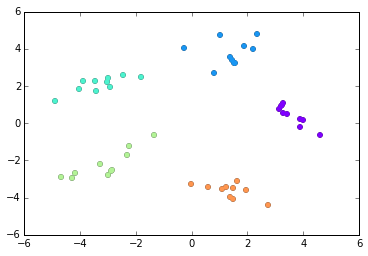
\includegraphics[scale=0.7]{images/kclustering.png} 
\caption{k-clustering of $50$ points into 5 clusters}

\end{figure}

These scripts are compiled with the option "scripts" of \texttt{setup.py} and should be callable from the shell. However in the near future the idea is to put them as modules callable from the \texttt{main} function of the package as a tutorial. 

\subsection{To Do list}
In this subsection we will put together all the aspects that need to be improved.
\begin{enumerate}
\item Tolerance Checking fast and reliable.
\item \texttt{main} function with scripts.
\item Good transformation from SDP into Conic Programming Problem.
\item More tests
\item Good input/output.
\end{enumerate}

\section{Documentation}
The package itself is not too large, thus the documentation is a simple \text{README.md} for github and a \text{README.txt} for pyPI and the installation. In it there are detailed explanations on how to install and run the package.

\section{Breakdown of the work}
Bernat Guillen: \texttt{SDP}, \texttt{DNNSDP}, \texttt{ConicProgrammingProblem} classes. \texttt{unittest} files. \texttt{points.py} script. All the structure of the package (including \texttt{setup.py}, \texttt{init} files, documentation and this report). Github: $72$ commits, $2640 ++, 1417--$

Michael Tarczon: First \texttt{C++} implementation of the solver but eventually discarded. Files \texttt{alignment.py} and \texttt{alignment.m} to compare results. Very valuable input on some issues of the coding regarding restrictions and SDP programming. Github: $12$ commits, $285++$, $113--$

Yuan Liu: Initially, interface between Python and C++, eventually discarded. Print method on \texttt{ConicProgrammingClass}. Github: $3$ commits, $29++$, $1--$

Special thanks to Yuehaw Khoo, who proposed the project back when we were 6 people in the team and was always available to solve doubts.

Although we would like to have a reasonable explanation of why there is a large disparity in the number of commits, we do not. A mix of bad luck (starting with a group of 6 people who then leave), personal problems, poor management skills... Whatever the reason is, I (Bernat Guillen) hope we all have learned from this not only how to code but also how to better plan group projects. In my opinion, this project had a lot of potential because SDP and Conic Programming are used now in a lot of applications and having 6 excellent people working on it would surely have resulted in a very interesting project. 

\section{Conclusions}

We have presented a package that implements the algorithm explained in \cite{sun2014} in \texttt{Python}. This package solves Conic Programming Problems, which include problems such as Semidefinite Programming and Doubly Non-Negative Semidefinite Programming. It is a fast algorithm with proof of convergence, the first of its kind that has a proof of convergence for problems with four sets of restrictions. Even though the package needs some improvements, it is fully functional and can be applied to many research problems now. 

\texttt{admm4block} can be installed using \texttt{pip} and also includes some example scripts, documentation and tests. It provides (in our opinion) a good balance between the flexibility a researcher needs and the easiness a regular user wants. 

It includes the classes 
\texttt{ConicProgrammingProblem} (for general problems), \texttt{SDP} and \texttt{DNNSDP} (for more specific problems). In the future it will include a User Interface and more kinds of problems such as LP or SOCP.


\begin{thebibliography}{9}

\bibitem{sun2014}
  {{Sun}, D. and {Toh}, K.-C. and {Yang}, L.},
  \emph{A Convergent 3-Block Semi-Proximal Alternating Direction Method of Multipliers for Conic Programming with 4-Type of Constraints}.
  ArXiv e-prints,
  1404.5378,
  2014.
\bibitem{pythondocs}
	{Ward, G. and Baxter, A.}
	"Distributing Python Modules". Python Software Foundation
	[URL:\url{https://docs.python.org/2/distutils/index.html}] Accessed Jan 14, 2015.
\bibitem{gitsym}
	"Symmetricity of SDP". Debate in github group.
	[URL:\url{https://github.com/cvxgrp/scs/issues/31}] Accessed Jan 15, 2015.
\end{thebibliography}


%%% End document
\end{document}
